\chapter{Data Fields and Example Data}

% \label{code:appendix-query-all-data}
\lstinputlisting[language=bash,
	caption={Query to fetch all Loan data from Kiva.org},
	label={code:appendix-query-all-data},
	basicstyle=\ttfamily\scriptsize,
	columns=fullflexible,
	breaklines=true,
	frame=single,
	postbreak=\mbox{\textcolor{red}{$\hookrightarrow$}\space},
]{artifacts/fetch_loans.graphql}

% /* cSpell:disable */ 
\begin{longtable}{|p{0.33\textwidth}|p{0.67\textwidth}|}
	\toprule\noalign{}
	\caption{Fields of Projects}
	\label{tab:appendix-fields-meaning}                                                                      \\

	\hline
	\multicolumn{1}{|c|}{\textbf{Field}} & \multicolumn{1}{c|}{\textbf{Meaning}}                             \\
	\hline
	\endfirsthead

	\multicolumn{2}{c}%
	{{\tablename\ \thetable{} -- continued from previous page}}                                              \\
	\hline
	\multicolumn{1}{|c|}{\textbf{Field}} & \multicolumn{1}{c|}{\textbf{Meaning}}                             \\
	\hline
	\endhead

	\hline
	\multicolumn{2}{|r|}{{Continued on next page}}                                                           \\ \hline
	\endfoot

	\hline \hline
	\endlastfoot

	activity                             & The activity is a structured categorization of the loan
	use                                                                                                      \\
	anonymizationLevel                   & The level of borrower privacy                                     \\
	borrowerCount                        & The number of borrowers participating in the loan                 \\
	borrowers                            & The one or more borrowers that are receiving this loan. If
	there is more than one, the primary borrower is first                                                    \\
	dafEligible                          & Whether or not the loan is eligible for donor-advised
	funds.                                                                                                   \\
	delinquent                           & Whether or not the loan is delinquent. This defaults to
	false if the user is not privileged to this loan                                                         \\
	description                          & The description of the loan profile in English.                   \\
	descriptionInOriginalLanguage        & The description of the loan profile in
	the original language of its posting                                                                     \\
	disbursalDate                        & The date on which the loan was/will actually be
	disbursed to the borrower                                                                                \\
	distributionModel                    & How the loan is distributed to the borrower,
	e.g.~`field\_partner' or `direct'                                                                        \\
	endorser                             & The user who endorsed the loan. Only shown on fundRaising
	loans, null for all other statuses.                                                                      \\
	fundraisingDate                      & When the loan started fundraising on Kiva. Same as
	posted\_date in v1.                                                                                      \\
	gender                               & The gender of the primary borrower OR majority gender if
	group                                                                                                    \\
	geocode                              & The physical location of the borrower and/or business             \\
	hasCurrencyExchangeLossLenders       & Whether or not the loan has currency
	loss to lenders. Only usable after the loan has moved into the ``ended''
	state.                                                                                                   \\
	id                                   & Unique identifier for a Kiva loan                                 \\
	image                                & The picture for this loan profile.                                \\
	isMatchable                          & Is this Kiva loan matchable? e.g.~is there a source of
	funds to provide matching if a share is purchased?                                                       \\
	inPfp                                & If true, this loan is in a Private Fundraising Period             \\
	loanAmount                           & The amount of this loan, as shown to lenders                      \\
	loanFundraisingInfo                  & Information about this loan during its fundraising
	period                                                                                                   \\
	lenderRepaymentTerm                  & The number of months it will take the borrower to
	repay the loan                                                                                           \\
	matcherAccountId                     & The id of the loan matcher                                        \\
	matcherName                          & The name of the loan matcher                                      \\
	matchRatio                           & The loan match ratio                                              \\
	matchingText                         & Text that is displayed if loan matching is turned on for
	this loan.                                                                                               \\
	name                                 & The name of the borrower or group receiving the loan              \\
	originalLanguage                     & The original language on the loan                                 \\
	minNoteSize                          & The minimum amount to lend for this loan                          \\
	paidAmount                           & The amount of settled repayments for a loan that has
	started paying back                                                                                      \\
	pfpMinLenders                        & The minimum number of lenders that this loan needs to
	exit its private fundraising period (PFP).                                                               \\
	plannedExpirationDate                & When the loan will expire if it is not fully
	funded                                                                                                   \\
	previousLoanId                       & ID of the loan linked as previous to this one.                    \\
	raisedDate                           & When the loan became raised, e.g.~fully funded. Same as
	funded\_date in v1                                                                                       \\
	researchScore                        & The research score of the loan theme instance of the
	loan                                                                                                     \\
	repaymentInterval                    & The repayment interval of the loan: ``monthly'',
	``irregularly'',``at\_end''                                                                              \\
	sector                               & The sector is a more general classification of the loan than
	activity                                                                                                 \\
	status                               & The status of a loan                                              \\
	tags                                 & A list of tags on this loan                                       \\
	terms                                & The financial terms of this loan                                  \\
	use                                  & Text describing what the loan is to be used for; a logical subset
	of description e.g.~``To buy a cow''                                                                     \\
	userProperties                       & Properties that apply to the logged in user in relation
	to a loan.                                                                                               \\
	video                                & Video for this loan                                               \\
	whySpecial                           & Why this loan is considered special.                              \\
	comments                             & List of A user comment made on a Kiva loan.                       \\
	lenders                              & List of Representation of a Kiva lender                           \\
	lendingActions                       & List of Representation of a lending action                        \\
	teams                                & List of Representation of a Kiva lending team                     \\
\end{longtable}


\begin{longtable}{|p{0.36\textwidth}|p{0.64\textwidth}|}
	\toprule\noalign{}
	\caption{An Example Project}
	\label{tab:appendix-example-data}                                                                                                                               \\

	\hline
	\multicolumn{1}{|c|}{\textbf{Field}}            & \multicolumn{1}{c|}{\textbf{Meaning}}                                                                         \\
	\hline
	\endfirsthead

	\multicolumn{2}{c}%
	{{\tablename\ \thetable{} -- continued from previous page}}                                                                                                     \\
	\hline
	\multicolumn{1}{|c|}{\textbf{Field}}            & \multicolumn{1}{c|}{\textbf{Meaning}}                                                                         \\
	\hline
	\endhead

	\hline
	\multicolumn{2}{|r|}{{Continued on next page}}                                                                                                                  \\
	\hline
	\endfoot

	\hline \hline
	\endlastfoot

	anonymizationLevel                              & none                                                                                                          \\
	borrowerCount                                   & 1                                                                                                             \\
	borrowers                                       & {[}\{`id': 2843387, `borrowedAmount': `440.80', `firstName':
	`Jessenia Elizabeth', `gender': `female', `isPrimary': True, `pictured':
	True\}{]}                                                                                                                                                       \\
	dafEligible                                     & False                                                                                                         \\
	delinquent                                      & False                                                                                                         \\
	disbursalDate                                   & 2013-09-25T07:00:00Z                                                                                          \\
	distributionModel                               & fieldPartner                                                                                                  \\
	endorser                                        &                                                                                                               \\
	fundraisingDate                                 & 2013-10-23T22:40:01Z                                                                                          \\
	gender                                          & female                                                                                                        \\
	hasCurrencyExchangeLossLenders                  & False                                                                                                         \\
	id                                              & 623042                                                                                                        \\
	isMatchable                                     & False                                                                                                         \\
	inPfp                                           & False                                                                                                         \\
	loanAmount                                      & 450.00                                                                                                        \\
	lenderRepaymentTerm                             & 8                                                                                                             \\
	matcherAccountId                                &                                                                                                               \\
	matcherName                                     &                                                                                                               \\
	matchRatio                                      &                                                                                                               \\
	matchingText                                    &                                                                                                               \\
	name                                            & Jessenia Elizabeth                                                                                            \\
	minNoteSize                                     & 25.00                                                                                                         \\
	paidAmount                                      & 0.00                                                                                                          \\
	pfpMinLenders                                   &                                                                                                               \\
	plannedExpirationDate                           & 2013-11-22T22:40:01Z                                                                                          \\
	previousLoanId                                  &                                                                                                               \\
	raisedDate                                      & 2013-10-24T13:38:51Z                                                                                          \\
	researchScore                                   & 9                                                                                                             \\
	repaymentInterval                               & monthly                                                                                                       \\
	status                                          & funded                                                                                                        \\
	tags                                            & {[}{]}                                                                                                        \\
	use                                             & purchase school supplies and other stationery items for her
	store.                                                                                                                                                          \\
	video                                           &                                                                                                               \\
	whySpecial                                      &                                                                                                               \\
	activity.id                                     & 103                                                                                                           \\
	activity.name                                   & Paper Sales                                                                                                   \\
	geocode.city                                    & Pichincha                                                                                                     \\
	geocode.state                                   & Pichincha                                                                                                     \\
	geocode.country.name                            & Ecuador                                                                                                       \\
	geocode.country.isoCode                         & EC                                                                                                            \\
	geocode.country.region                          & South America                                                                                                 \\
	geocode.country.ppp                             & \$10,600                                                                                                      \\
	geocode.country.\densetext{numLoansFundraising} & 553                                                                                                           \\
	geocode.country.fundsLentInCountry              & 87573245                                                                                                      \\
	geocode.postalCode                              &                                                                                                               \\
	geocode.latitude                                & -0.1464847                                                                                                    \\
	geocode.longitude                               & -78.4751945                                                                                                   \\
	image.id                                        & 1456025                                                                                                       \\
	image.url                                       &
	\href{https://www-kiva-org-0.freetls.fastly.net/img/s100/5cf86ba6c72db94f0721b934a57ca889.jpg}{https://www-kiva-org-0.freetls.fastly.net/img/s100/5cf86ba6c...} \\
	loanFundraisingInfo.fundedAmount                & 450.00                                                                                                        \\
	loanFundraisingInfo.isExpiringSoon              & False                                                                                                         \\
	loanFundraisingInfo.reservedAmount              & 0.00                                                                                                          \\
	originalLanguage.id                             & 2                                                                                                             \\
	originalLanguage.isActive                       & True                                                                                                          \\
	originalLanguage.isoCode                        & ES                                                                                                            \\
	originalLanguage.name                           & Spanish                                                                                                       \\
	sector.id                                       & 7                                                                                                             \\
	sector.name                                     & Retail                                                                                                        \\
	terms.currency                                  & USD                                                                                                           \\
	terms.currencyFullName                          & United States Dollars                                                                                         \\
	terms.disbursalAmount                           & 440.80                                                                                                        \\
	terms.disbursalDate                             & 2013-09-25T07:00:00Z                                                                                          \\
	terms.expectedPayments                          & {[}{]}                                                                                                        \\
	terms.loanAmount                                & 450.00                                                                                                        \\
	terms.lenderRepaymentTerm                       & 8                                                                                                             \\
	terms.lossLiabilityCurrencyExchange             & none                                                                                                          \\
	terms.lossLiabilityNonpayment                   & lender                                                                                                        \\
	terms.flexibleFundraisingEnabled                & False                                                                                                         \\
	userProperties.favorited                        &                                                                                                               \\
	userProperties.lentTo                           &                                                                                                               \\
	userProperties.subscribed                       &                                                                                                               \\
	userProperties.promoEligible                    & False                                                                                                         \\
	userProperties.amountInBasket                   &                                                                                                               \\
	lendingActions.totalCount                       & 14                                                                                                            \\
	lendingActions.values                           & {[}\{`lender': \{`id': 32817, `name': `Nate',
	`publicId': `nateinaction'\}, `shareAmount': `25.00', `teams': {[}`(A+)
	Atheists'{]}, `latestSharePurchaseDate': `2013-10-24T11:50:07Z'\},
	\{`lender': \{`id': 55596, `name': `Dirk L.', `publicId': `DirkLebe'\},
	`shareAmount': `25.00', `teams': {[}{]}, `latestSharePurchaseDate':
	`2013-10-24T02:40:53Z'\}{]}                                                                                                                                     \\
	description                                     & Every fifteen days, the members of the Community Bank of
	Pichincha meet in their home region of Pichincha. This area is well
	known as a vibrant place, where the majority of the people are farmers
	or ranchers. It's a highly vegetated area, cut by a great river that
	nurtures the crops.                                                                                                                                             \\
	                                                & This is where Jessenia, 27 years old, lives with her common-law
	husband and their three children, aged 9, 4, and 2 years. The eldest is
	a student, and her husband is a shopkeeper.Jessenia is a woman with
	spirit who likes to work to get ahead. For the last six years, she has
	run a shop out of her home that functions as a stationery shop and a
	bookstore. Day by day, the store has improved. Currently, apart from
	books and supplies, she also sells trinkets and other school/office
	supplies. With these products, her earnings have greatly increased, and
	thanks to the loans she has received, she has been able to expand her
	business.                                                                                                                                                       \\
	                                                & This loan will be used to buy school supplies and other stationery
	products. She has been in the Community Bank for eight years and she
	likes it because the loans have helped her improve her business. She
	dreams of expanding it further still.                                                                                                                           \\
	descriptionInOriginalLanguage                   & En el cantón Pichincha cada quince días
	se reúne el Banco Comunal Pichincha, este lugar se lo conoce por ser muy
	dinámico donde la mayoría de sus habitantes se dedican a la agricultura
	y a la cría de animales, por ser una zona con gran vegetación surcada
	por un gran rio lo cual lo hace propicia para los cultivos.                                                                                                     \\
	                                                & En este lugar vive la señora Jessenia, tiene 27 años de edad y
	mantiene una relación de unión libre de la cual tiene tres hijos de 9, 4
	y 2 años de edad, el mayor estudia en escuela. El marido es
	comerciante.                                                                                                                                                    \\
	                                                & Doña Jessenia es una mujer muy luchadora que le gusta trabajar para
	salir adelante, ella hace mas de 6 años adecuo un local en su casa y en
	el mismo instaló una papelería y librería, la misma que con el paso de
	los días ha ido mejorando, actualmente además de libros y útiles también
	vende bisutería y artículos de bazar con esto sus ganancias han mejorado
	mucho y esto gracias a los créditos que ha recibido ya que con ellos
	cada vez aumenta más su negocio.                                                                                                                                \\
	                                                & Este crédito es para comprar útiles escolares y artículos de bazar.
	Esta desde hace 8 años en el Banco Comunal y le gusta porque los
	créditos le han ayudado a mejora su negocio. Sus sueños son aumentar más
	su negocio.
\end{longtable}


\begin{longtable}[]{|r|l|r|l|r|l|}

	\toprule\noalign{}
	\caption{List of Activities}
	\label{tab:appendix-activity-definition}                                                                                 \\

	\hline
	\textbf{id} & \textbf{Name}         & \textbf{id} & \textbf{Name}             & \textbf{id} & \textbf{Name}              \\
	\hline
	\endfirsthead

	\multicolumn{6}{c}%
	{{\tablename\ \thetable{} -- continued from previous page}}                                                              \\
	\hline
	\textbf{id} & \textbf{Name}         & \textbf{id} & \textbf{Name}             & \textbf{id} & \textbf{Name}              \\
	\hline
	\endhead

	\hline
	\multicolumn{6}{|r|}{{Continued on next page}}                                                                           \\
	\hline
	\endfoot

	\hline \hline
	\endlastfoot


	9           & Clothing Sales        & 84          & Used Clothing             & 147         & Well digging               \\
	11          & Land Rental           & 85          & Laundry                   & 149         & Embroidery                 \\
	12          & Traveling Sales       & 86          & Textiles                  & 151         & Music Discs \& Tapes       \\
	13          & Veterinary Sales      & 87          & Food Market               & 156         & Rickshaw                   \\
	14          & Bookstore             & 88          & Retail                    & 157         & Call Center                \\
	15          & Grocery Store         & 89          & Fishing                   & 158         & Primary/secondary school
	costs                                                                                                                    \\
	17          & Musical Performance   & 91          & Milk Sales                & 159         & Bookbinding                \\
	18          & Water Distribution    & 92          & Auto Repair               & 161         & Movie Tapes \&
	DVDs                                                                                                                     \\
	19          & Cosmetics Sales       & 94          & Pub                       & 162         & Liquor Store / Off-License \\
	21          & Bicycle Repair        & 95          & Machine Shop              & 163         & Waste Management           \\
	23          & Shoe Sales            & 96          & Phone Accessories         & 164         & Film                       \\
	24          & Construction Supplies & 97          & Cement                    & 165         & Knitting                   \\
	25          & Cafe                  & 98          & Decorations Sales         & 167         & Upholstery                 \\
	26          & Plastics Sales        & 99          & Pigs                      & 169         & Fruits \& Vegetables       \\
	27          & Bakery                & 100         & Phone Repair              & 170         & Jewelry                    \\
	28          & Barber Shop           & 101         & Cobbler                   & 171         & Cloth \& Dressmaking
	Supplies                                                                                                                 \\
	29          & Home Products Sales   & 102         & Poultry                   & 172         & Internet Cafe              \\
	31          & Farming               & 103         & Paper Sales               & 174         & Entertainment              \\
	32          & Tailoring             & 104         & Electronics Repair        & 175         & Games                      \\
	33          & Furniture Making      & 105         & Air Conditioning          & 176         & Education
	provider                                                                                                                 \\
	34          & Butcher Shop          & 107         & Transportation            & 177         & Flowers                    \\
	35          & Cheese Making         & 108         & Blacksmith                & 180         & Wholesale                  \\
	37          & Motorcycle Transport  & 109         & Perfumes                  & 181         & Food                       \\
	39          & Construction          & 110         & Animal Sales              & 183         & Clothing                   \\
	40          & Phone Use Sales       & 111         & Computers                 & 184         & Machinery Rental           \\
	41          & Sporting Good Sales   & 112         & Cereals                   & 185         & Food Stall                 \\
	43          & Carpentry             & 114         & Secretarial Services      & 186         & Balut-Making               \\
	45          & Catering              & 115         & Dental                    & 192         & Personal Medical Expenses  \\
	46          & Restaurant            & 116         & Electrician               & 193         & Property                   \\
	47          & Sewing                & 117         & Mobile Phones             & 194         & Consumer Goods             \\
	49          & Beauty Salon          & 119         & Quarrying                 & 195         & Home Appliances            \\
	51          & Electronics Sales     & 120         & Agriculture               & 196         & Vehicle                    \\
	52          & Metal Shop            & 121         & Services                  & 197         & Wedding Expenses           \\
	54          & Vehicle Repairs       & 123         & Health                    & 199         & Used Shoes                 \\
	56          & Cattle                & 124         & Manufacturing             & 200         & Higher education costs     \\
	57          & General Store         & 125         & Arts                      & 201         & Renewable Energy Products  \\
	59          & Taxi                  & 127         & Party Supplies            & 202         & Recycled Materials         \\
	60          & Charcoal Sales        & 128         & Timber Sales              & 203         & Home Energy                \\
	61          & Dairy                 & 129         & Child Care                & 204         & Cleaning Services          \\
	62          & Photography           & 130         & Fuel/Firewood             & 206         & Communications             \\
	63          & Fish Selling          & 131         & Electrical Goods          & 207         & Adult Care                 \\
	65          & Pharmacy              & 132         & Religious Articles        & 208         & Energy                     \\
	66          & Printing              & 133         & Tourism                   & 209         & Florist                    \\
	67          & Food Production/Sales & 134         & Personal Housing Expenses & 210         &
	Landscaping / Gardening                                                                                                  \\
	68          & Farm Supplies         & 135         & Motorcycle Repair         & 216         & Technology                 \\
	70          & Medical Clinic        & 137         & Utilities                 & 217         & Beekeeping                 \\
	72          & Crafts                & 138         & Recycling                 & 218         & Aquaculture                \\
	73          & Livestock             & 140         & Souvenir Sales            & 219         & Computer                   \\
	75          & Patchwork             & 141         & Spare Parts               & 220         & Beverages                  \\
	76          & Bicycle Sales         & 142         & Personal Products Sales   & 221         & Personal Care
	Products                                                                                                                 \\
	78          & Musical Instruments   & 143         & Natural Medicines         & 222         & Funerals                   \\
	79          & Bricks                & 144         & Goods Distribution        & 223         & Celebrations               \\
	80          & Office Supplies       & 145         & Weaving                   & 224         & Personal Expenses          \\
	81          & Hardware              & 146         & Hotel                     & 225         & Mobile Transactions        \\
	            &                       &             &                           & 226         & Event Planning             \\
\end{longtable}


\begin{longtable}{|r|l|l|r|l|l|}
	\toprule\noalign{}
	\caption{List of Tags}
	\label{tab:appendix-tag-definition}                                                                                                                                      \\

	\hline
	\textbf{id} & \textbf{name}                    & \densetext{\textbf{vocabularyId}} & \textbf{id} & \textbf{name}                     & \densetext{\textbf{vocabularyId}} \\
	\hline
	\endfirsthead

	\multicolumn{6}{c}%
	{{\tablename\ \thetable{} -- continued from previous page}}                                                                                                              \\
	\hline
	\textbf{id} & \textbf{name}                    & \densetext{\textbf{vocabularyId}} & \textbf{id} & \textbf{name}                     & \densetext{\textbf{vocabularyId}} \\
	\hline
	\endhead

	\hline
	\multicolumn{6}{|r|}{{Continued on next page}}                                                                                                                           \\
	\hline
	\endfoot

	\hline \hline
	\endlastfoot
	1           & volunteer\_pick                  & 1                                 & 20          & \#Post-disbursed                  & 2                                 \\
	2           & volunteer\_like                  & 1                                 & 21          & \#Inspiring Story                 & 2                                 \\
	3           & user\_like                       & 1                                 & 14          & \#Single                          & 2                                 \\
	4           & user\_favorite                   & 1                                 & 23          & \#Interesting Photo               & 2                                 \\
	26          & \#Fabrics                        & 2                                 & 66          & \#TangibleProducts                & 3                                 \\
	27          & \#Health and Sanitation          & 2                                 & 61          & \#Agriculture                     & 3                                 \\
	28          & \#Repeat Borrower                & 2                                 & 62          & \#NewBusiness                     & 3                                 \\
	29          & \#Refugee                        & 2                                 & 63          & \#Values                          & 3                                 \\
	30          & \#Job Creator                    & 2                                 & 64          & \#PersonalImpact                  & 3                                 \\
	31          & \#Supporting Family              & 2                                 & 65          & \#QualityPhotos                   & 3                                 \\
	32          & \#Orphan                         & 2                                 & 73          & LGBTQ                             & 3                                 \\
	33          & \#Low-profit FP                  & 2                                 & 68          & \#StandoutBackstory               & 3                                 \\
	35          & \#Biz Durable Asset              & 2                                 & 69          & \#UniqueLoanUse                   & 3                                 \\
	25          & \#Team Guys Holding Fish         & 2                                 & 70          & MUFG                              & 3                                 \\
	36          & \#Trees                          & 2                                 & 71          & LISCChicago                       & 3                                 \\
	37          & \#Female Education               & 2                                 & 72          & \#Kaiser                          & 3                                 \\
	39          & \#Repair Renew Replace           & 2                                 & 60          & \#Refugees                        & 3                                 \\
	40          & \#US immigrant                   & 2                                 & 74          & US Refugee                        & 3                                 \\
	43          & \#US Black-Owned Business        & 2                                 & 67          & \#HighDetail                      & 3                                 \\
	45          & \#Latinx/Hispanic-Owned Business & 2                                 & 59          & \#COVID-19                        & 3                                 \\
	34          & \#Hidden Gem                     & 2                                 & 50          & GoDaddy                           & 3                                 \\
	24          & \#Powerful Story                 & 2                                 & 57          & \#GenderEquity                    & 3                                 \\
	38          & \#Technology                     & 2                                 & 75          & Viral                             & 3                                 \\
	22          & \#Unique                         & 2                                 & 41          & reserved\_disaster\_relief\_covid & 3                                 \\
	5           & \#First Loan                     & 2                                 & 42          & reserved\_crisis\_support\_loan   & 3                                 \\
	6           & \#Woman-Owned Business           & 2                                 & 44          &                                   & 3                                 \\
	7           & \#Tourism                        & 2                                 & 46          & cow                               & 3                                 \\
	8           & \#Sustainable Ag                 & 2                                 & 47          & IT Cosmetics                      & 3                                 \\
	9           & \#Eco-friendly                   & 2                                 & 58          & \#Education                       & 3                                 \\
	11          & \#Animals                        & 2                                 & 48          & beauty                            & 3                                 \\
	12          & \#Widowed                        & 2                                 & 51          & \#BIPOC-owned Business            & 3                                 \\
	13          & \#Elderly                        & 2                                 & 52          & \#Umpqua                          & 3                                 \\
	10          & \#Vegan                          & 2                                 & 53          & \#US Environmental Loan           & 3                                 \\
	15          & \#Married                        & 2                                 & 54          & \#CommunityImpact                 & 3                                 \\
	16          & \#Parent                         & 2                                 & 55          & \#FamilyImpact                    & 3                                 \\
	17          & \#Single Parent                  & 2                                 & 56          & \#EcoFriendly                     & 3                                 \\
	18          & \#Schooling                      & 2                                 & 49          & Turo                              & 3                                 \\
	19          & \#Pre-disbursed                  & 2                                 & 76          & Salesforce                        & 3                                 \\
\end{longtable}
%/* cSpell:enable */   

\chapter{Data overview}

% /* cSpell:disable */
\begin{longtable}{|c|l|r|r|c|l|r|r|}
	\toprule\noalign{}
	\caption{Distribution of Projects by Countries}
	\label{tab:appendix-project-vs-country}                                                                                                                                                                                 \\

	\hline
	\textbf{No} & \textbf{country name} & \densetext{\textbf{project count}} & \densetext{\textbf{avg amount}} & \textbf{No} & \textbf{country name} & \densetext{\textbf{project count}} & \densetext{\textbf{avg amount}} \\
	\hline
	\endfirsthead

	\multicolumn{8}{c}%
	{{\tablename\ \thetable{} -- continued from previous page}}                                                                                                                                                             \\
	\hline
	\textbf{No} & \textbf{country name} & \densetext{\textbf{project count}} & \densetext{\textbf{avg amount}} & \textbf{No} & \textbf{country name} & \densetext{\textbf{project count}} & \densetext{\textbf{avg amount}} \\
	\hline
	\endhead

	\hline
	\multicolumn{8}{|r|}{{Continued on next page}}                                                                                                                                                                          \\
	\hline
	\endfoot

	\hline \hline
	\endlastfoot
	1           & Philippines           & 219376                             & 353.69                          & 47          & Fiji                  & 4168                               & 806.3                           \\
	2           & Kenya                 & 129479                             & 520.18                          & 48          & Costa Rica            & 3911                               & 1296.77                         \\
	3           & El Salvador           & 49085                              & 690.84                          & 49          & Solomon Islands       & 3463                               & 812.29                          \\
	4           & Tajikistan            & 43283                              & 811.66                          & 50          & Lesotho               & 2795                               & 356.43                          \\
	5           & Cambodia              & 42828                              & 577.72                          & 51          & Tonga                 & 2465                               & 1637.51                         \\
	6           & Ecuador               & 34689                              & 1128.59                         & 52          & Cameroon              & 2427                               & 464.86                          \\
	7           & Uganda                & 34472                              & 814.55                          & 53          & Myanmar (Burma)       & 2269                               & 1807.44                         \\
	8           & Colombia              & 31730                              & 642.87                          & 54          & Moldova               & 2088                               & 2071.74                         \\
	9           & Pakistan              & 30633                              & 515.91                          & 55          & Kosovo                & 1870                               & 1418.55                         \\
	10          & Nicaragua             & 21661                              & 973.53                          & 56          & Malawi                & 1851                               & 1826.02                         \\
	11          & Peru                  & 20810                              & 1779.7                          & 57          & Zambia                & 1556                               & 1641.69                         \\
	12          & Vietnam               & 20160                              & 1299.59                         & 58          & Azerbaijan            & 1458                               & 1606.86                         \\
	13          & Madagascar            & 18572                              & 287.9                           & 59          & Brazil                & 1423                               & 2440.41                         \\
	14          & Paraguay              & 17910                              & 2617.26                         & 60          & Dominican Republic    & 1417                               & 2571.18                         \\
	15          & Indonesia             & 15344                              & 533.95                          & 61          & Yemen                 & 1253                               & 892.1                           \\
	16          & Lebanon               & 14512                              & 1344.55                         & 62          & Vanuatu               & 1048                               & 726.57                          \\
	17          & Kyrgyzstan            & 14036                              & 1295.9                          & 63          & Lao PDR               & 1047                               & 654.56                          \\
	18          & Samoa                 & 12912                              & 862.07                          & 64          & Thailand              & 1007                               & 2479.5                          \\
	19          & India                 & 11737                              & 640.91                          & 65          & Mongolia              & 961                                & 1776.09                         \\
	20          & Palestine             & 11333                              & 1993.99                         & 66          & Ukraine               & 808                                & 1881.66                         \\
	21          & Togo                  & 11172                              & 414.21                          & 67          & Nepal                 & 652                                & 689.57                          \\
	22          & Guatemala             & 11139                              & 2516.16                         & 68          & Burundi               & 557                                & 3249.11                         \\
	23          & Nigeria               & 10823                              & 308.52                          & 69          & Iraq                  & 526                                & 3580.17                         \\
	24          & Honduras              & 10754                              & 1037.36                         & 70          & Papua New Guinea      & 413                                & 998.24                          \\
	25          & Rwanda                & 10721                              & 3354.82                         & 71          & Panama                & 361                                & 2512.38                         \\
	26          & Bolivia               & 10354                              & 2749.46                         & 72          & Israel                & 347                                & 4654.93                         \\
	27          & Senegal               & 10191                              & 2626.79                         & 73          & Puerto Rico           & 323                                & 7854.58                         \\
	28          & Liberia               & 9662                               & 471.61                          & 74          & Benin                 & 278                                & 1888.81                         \\
	29          & Sierra Leone          & 9434                               & 779.79                          & 75          & South Africa          & 252                                & 2000.1                          \\
	30          & Jordan                & 9255                               & 1157.21                         & 76          & Suriname              & 178                                & 2610.98                         \\
	31          & United States         & 8489                               & 6288.98                         & 77          & China                 & 83                                 & 3195.54                         \\
	32          & Ghana                 & 8113                               & 1218.29                         & 78          & Congo                 & 73                                 & 6222.49                         \\
	33          & Armenia               & 7765                               & 1515.62                         & 79          & Somalia               & 52                                 & 3931.18                         \\
	34          & Tanzania              & 7617                               & 1260.73                         & 80          & South Sudan           & 38                                 & 8014.33                         \\
	35          & Timor-Leste           & 7260                               & 871.11                          & 81          & Belize                & 33                                 & 862.5                           \\
	36          & Mexico                & 7044                               & 1633.42                         & 82          & Namibia               & 28                                 & 26954.48                        \\
	37          & Congo (DRC)           & 6431                               & 4078.6                          & 83          & Bangladesh            & 25                                 & 42482.28                        \\
	38          & Zimbabwe              & 6077                               & 877.53                          & 84          & Chile                 & 7                                  & 18105.88                        \\
	39          & Burkina Faso          & 5876                               & 1172.89                         & 85          & St Vincent            & 5                                  & 3630.56                         \\
	40          & Mozambique            & 5460                               & 846.06                          & 86          & Cote D'Ivoire         & 4                                  & 25928.12                        \\
	41          & Haiti                 & 4695                               & 1107.43                         & 87          & Afghanistan           & 2                                  & 6923.08                         \\
	42          & Georgia               & 4542                               & 1466.06                         & 88          & Guam                  & 2                                  & 4333.33                         \\
	43          & Egypt                 & 4535                               & 856.04                          & 89          & Bhutan                & 1                                  & 10000.0                         \\
	44          & Turkey                & 4513                               & 365.14                          & 90          & Canada                & 1                                  & 50000.0                         \\
	45          & Mali                  & 4249                               & 2157.97                         & 91          & Mauritania            & 1                                  & 15000.0                         \\
	46          & Albania               & 4233                               & 1669.89                         & 92          & Sri Lanka             & 1                                  & 450.0                           \\
	            &                       &                                    &                                 & 93          & Uruguay               & 1                                  & 8000.0                          \\
\end{longtable}


\begin{longtable}{|c|l|r|r|}
	\toprule\noalign{}
	\caption{Distribution of Projects by Tags}
	\label{tab:appendix-project-vs-tag}                                                                    \\

	\hline
	\textbf{No} & \textbf{Tag}                     & \textbf{Project count} & \textbf{Average Loan Amount} \\
	\hline
	\endfirsthead

	\multicolumn{4}{c}%
	{{\tablename\ \thetable{} -- continued from previous page}}                                            \\
	\hline
	\textbf{No} & \textbf{Tag}                     & \textbf{Project count} & \textbf{Average Loan Amount} \\
	\hline
	\endhead

	\hline
	\multicolumn{4}{|r|}{{Continued on next page}}                                                         \\
	\hline
	\endfoot

	\hline \hline
	\endlastfoot

	1           & \#Woman-Owned Business           & 525767                 & 943.48                       \\
	2           & \#Parent                         & 464637                 & 889.20                       \\
	3           & \#Repeat Borrower                & 250713                 & 993.38                       \\
	4           & \#Elderly                        & 171442                 & 781.28                       \\
	5           & \#Animals                        & 140633                 & 816.53                       \\
	6           & \#Eco-friendly                   & 126065                 & 767.86                       \\
	7           & \#Schooling                      & 122842                 & 934.43                       \\
	8           & \#Vegan                          & 103935                 & 934.96                       \\
	9           & \#Health and Sanitation          & 90618                  & 630.69                       \\
	10          & \#Biz Durable Asset              & 87061                  & 1265.14                      \\
	11          & \#Technology                     & 65557                  & 725.45                       \\
	12          & \#Single Parent                  & 55925                  & 989.94                       \\
	13          & \#Supporting Family              & 53536                  & 936.91                       \\
	14          & \#Fabrics                        & 52927                  & 1096.92                      \\
	15          & \#Single                         & 48513                  & 935.22                       \\
	16          & \#First Loan                     & 43115                  & 1118.88                      \\
	17          & \#Repair Renew Replace           & 38795                  & 994.39                       \\
	18          & \#Widowed                        & 31518                  & 902.32                       \\
	19          & \#Sustainable Ag                 & 30746                  & 1130.55                      \\
	20          & \#Job Creator                    & 19772                  & 1819.23                      \\
	21          & \#Female Education               & 16491                  & 1091.24                      \\
	22          & \#Trees                          & 16439                  & 1196.81                      \\
	23          & \#Refugee                        & 14033                  & 1409.83                      \\
	24          & \#Unique                         & 9720                   & 3362.81                      \\
	25          & \#Low-profit FP                  & 7286                   & 1265.20                      \\
	26          & \#Interesting Photo              & 5897                   & 1274.42                      \\
	27          & \#BIPOC-owned Business           & 5523                   & 5900.62                      \\
	28          & \#Inspiring Story                & 4635                   & 1889.90                      \\
	29          & \#US Black-Owned Business        & 3075                   & 5897.17                      \\
	30          & \#Post-disbursed                 & 2719                   & 1670.03                      \\
	31          & \#Latinx/Hispanic-Owned Business & 2104                   & 5064.92                      \\
	32          & \#Umpqua                         & 1757                   & 5362.56                      \\
	33          & \#Hidden Gem                     & 1541                   & 1752.11                      \\
	34          & \#US immigrant                   & 1533                   & 5526.88                      \\
	35          & \#Orphan                         & 877                    & 1722.18                      \\
	36          & LGBTQ                            & 304                    & 7133.22                      \\
	37          & \#Tourism                        & 203                    & 1402.46                      \\
	38          & US Refugee                       & 136                    & 6966.91                      \\
	39          & \#Team Guys Holding Fish         & 120                    & 1311.67                      \\
	40          & \#Married                        & 102                    & 1752.21                      \\
	41          & \#TangibleProducts               & 93                     & 8956.99                      \\
	42          & \#CommunityImpact                & 81                     & 9030.86                      \\
	43          & \#Powerful Story                 & 48                     & 3316.67                      \\
	44          & \#EcoFriendly                    & 29                     & 10810.34                     \\
	45          & Viral                            & 21                     & 9860.71                      \\
	46          & \#US Environmental Loan          & 19                     & 8868.42                      \\
	47          & \#Education                      & 16                     & 7218.75                      \\
	48          & \#Agriculture                    & 14                     & 9178.57                      \\
	49          & \#StandoutBackstory              & 12                     & 9041.67                      \\
	50          & \#NewBusiness                    & 11                     & 7363.64                      \\
	51          & MUFG                             & 9                      & 6888.89                      \\
	52          & \#Kaiser                         & 5                      & 13500.00                     \\
	53          & \#GenderEquity                   & 4                      & 15625.00                     \\
	54          & beauty                           & 3                      & 1216.67                      \\
	55          & cow                              & 3                      & 1475.00                      \\
	56          & \#COVID-19                       & 2                      & 11250.00                     \\
	57          & \#Pre-disbursed                  & 1                      & 5950.00                      \\
	58          & GoDaddy                          & 1                      & 10000.00                     \\
	59          & LISCChicago                      & 1                      & 9500.00                      \\
\end{longtable}
% /* cSpell:enable */

\chapter{Data synthesis algorithms}

\begin{algorithm}
	\noindent
	\caption{Synthesis graph nodes generation}
	\label{alg:appendix-synthesis_graph_nodes}
	\begin{description}
		\item[Input:] number of time step $T$
		\item[\phantom{Input:}] number of nodes $n$
		\item[\phantom{Input:}] number of community $c$
		\item[\phantom{Input:}] probability a node stay in a same community in one step $p_{stay}$
		\item[Output:] community indexes $C \in \mathbb{N}^{T \times n \times c}$
	\end{description}
	\begin{algorithmic}[1]
		\Function{generate\_community\_dynamic}{$n, c, T$}
		\For {$i = 1,2,\ldots,n$}
		\Comment Init randomly for the first time step
		\State $C[1][i] \gets$ \Call{random\_integer}{$1, c$}
		\EndFor
		\For {$t = 2,3,\ldots,T$}
		\For {$i = 1,2,\ldots,n$}
		\If{\Call{random} $\le p_{stay}$}
		\State $C[t][i] \gets C[t-1][i]$
		\Comment Stay in the same community
		\Else
		\State $C[t][i] \gets$ \Call{random\_integer}{$1, c$}
		\Comment Change to a new community randomly
		\EndIf
		\EndFor
		\EndFor
		\State \textbf{return} $C$
		\EndFunction
	\end{algorithmic}
\end{algorithm}


\begin{algorithm}
	\caption{Synthesis graph co-cluster generation}
	\label{alg:appendix-synthesis_graph_cocluster}
	\begin{description}
		\item[Input:] number of cluster $c_1, c_2$
		\item[Output:] map $M$ from $[1, 2, \ldots, \max(c_1, c_2)]$ to $[1, 2, \ldots, \max(c_1, c_2)]$
	\end{description}
	\begin{algorithmic}[1]
		\Function{generate\_cocluster}{$c_1, c_2$}
		\For{$i=1,2,\ldots,\min(c_1, c_2)$}
		\State $M[i] \gets i$
		\EndFor
		\For{$i=\min(c_1, c_2)+1, \ldots, \max(c_1, c_2)$}
		\State $M[i] \gets$ \Call{random\_integer}{$1, \min(c_1, c_2)$}
		\EndFor
		\EndFunction
	\end{algorithmic}
	\begin{algorithmic}[1]
		\Function{is\_same\_cocluster}{$c_1, c_2$}
		\State \textbf{return} $M[c_1] = c_2$ \textbf{or} $M[c_2] = c_1$
		\EndFunction
	\end{algorithmic}
\end{algorithm}


\algnewcommand\algorithmicforeach{\textbf{for each}}
\algdef{S}[FOR]{ForEach}[1]{\algorithmicforeach\ #1\ \algorithmicdo}

\begin{algorithm}
	\noindent
	\caption{Synthesis graph edges generation}
	\label{alg:appendix-synthesis_graph_edges}
	\begin{description}
		\item[Input/Output: ] biadjacency matrix $B \in \mathbb{R}^{n_1 \times n_2}$
		\item[Input:] $V_1$ community index $C \in \mathbb{N}^{n_1}$
		\item[\phantom{Input:}] $V_2$ community index $D \in \mathbb{N}^{n_2}$
		\item[\phantom{Input:}] $c_1, c_2, p_{in}, p_{out}$
	\end{description}
	\begin{algorithmic}[1] % line number
		\Function{generate\_edges}{$B, C, D, c_1, c_2, p_{in}, p_{out}$}
		\ForEach{$(i, j)$ \textbf{in} $[1, 2, \ldots, n_1] \times [1, 2, \ldots, n_2]$}
		\If{\Call{is\_same\_cocluster}{$C[i], D[j]$}}
		\If{\Call{random} $\le p_{in}$}
		\State $B[i][j] \gets 1$
		\EndIf
		\Else
		\If{\Call{random} $\le p_{out}$}
		\State $B[i][j] \gets 1$
		\EndIf
		\EndIf
		\EndFor
		\EndFunction
	\end{algorithmic}

\end{algorithm}


\chapter{Community detection results}

\begin{figure}[H]
	\centering
	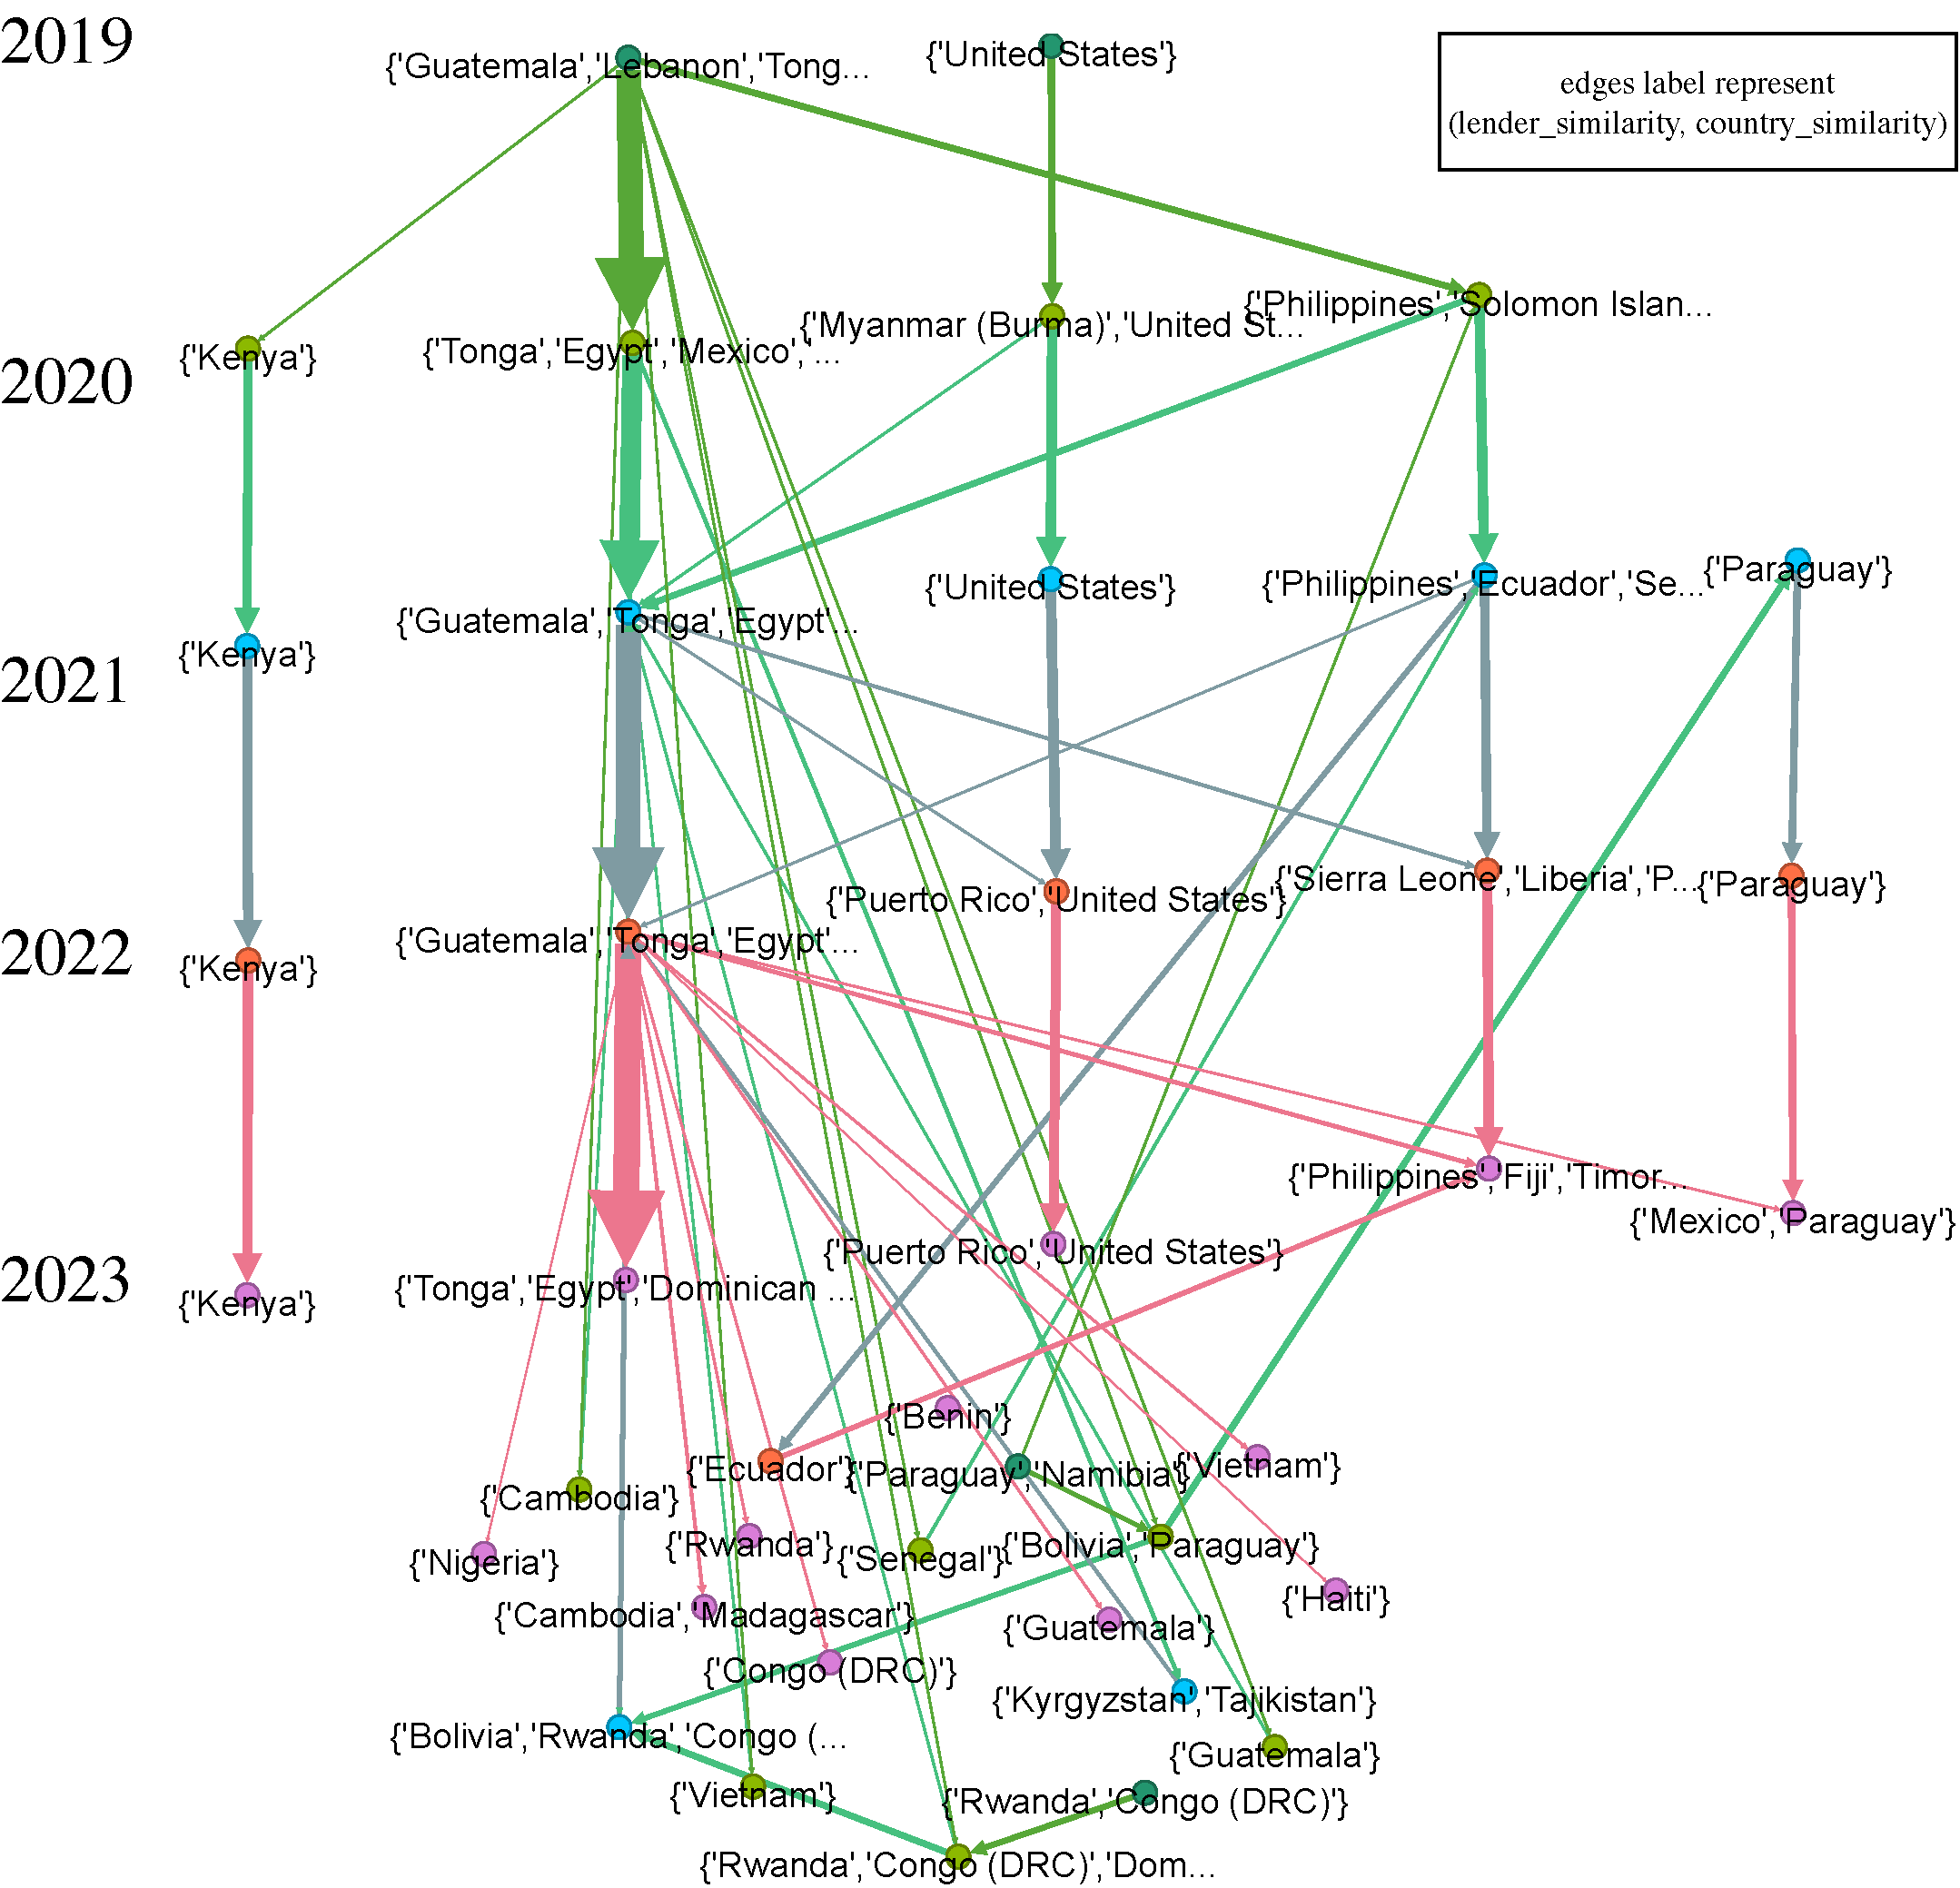
\includegraphics[width=0.8\textwidth]{images/LCountry-full.pdf}
	\caption[Illustrate the result of Lender-Country community detection]{
		Illustrate the result of Lender-Country community detection.
		Each edges is a tuple of similarities between Lender nodes and Country nodes over the years.
		The thickness of the edge is proportional to the minimum similarity $min(\text{lender\_similarity}, \text{sector\_similarity})$.
		All edges is shown.
	}
	\label{fig:appendix-LCountry-full}
\end{figure}
